%-------------------------------------------------------------------------------------------------%
% A related work section in which the relevant literature is presented and 
% linked to the project. 
% It should show that you clearly know the problem you plan to solve, 
% and that you master the related work. 
%
% Ken: flip this upside down
% start out with the generalities
% go into the specifics
% 
% 

\newpage

\section{Related work}

This chapter offers background literature on the aforementioned topics, and will explain how this literature relates to the proposed study. three related topics are regarded: prior studies on WebAssembly, Prior studies on client-side geoprocessing, and prior studies on geoprocessing interfaces.



\subsection{WebAssembly \& Geoprocessing performance}

The aims of the proposed thesis require us to be aware of the state of the art of WebAssembly, its performance considerations, and how this relates to geoprocessing performance. But first, an introduction on the compilation target itself is in order.

The original paper on WebAssembly was published on June 14, 2017 \cite{haas_bringing_2017}. The authors write that the reason behind the creation of WebAssembly is the observation that certain high-end applications started using JavaScript as a compile target, using a high-performance subset of javascript \cite{mozilla_asmjs_2013}. However, JavaScript remains a high-level, highly abstract programming language, which never intended to be used as a compile target. The discrepancy between intended use and actual use led to many complications for developers using javascript this way, but also for the developers of javascript itself \cite{haas_bringing_2017}. This is why developers of the four major browser vendors Mozilla, Google, Apple and Microsoft eventually joined up, and created WebAssembly and its corresponding paper. %all in order to relieve javascript of the responsibility of being a low-level compilation target. 

This paper starts by promising WebAssembly as a save, fast, portable and compact compilation target. It continues by showing how previous attempts at low-level code on the web fail in at least one of these criteria, and that WebAssembly is the first to deliver on all of them. The follow up chapters cover a proof of memory safety, a proof of soundness of the language design, and the design decisions which had to be made to live up to those four criteria. These details will become relevant to the proposed thesis when reasoning about why WebAssembly might be faster in one case versus another.

\subsubsection*{Performance}

The initial performance benchmarks look promising. A the majority of performance comparisons show a WebAssembly only taking 10\% longer than the native binary it was compared to \cite{haas_bringing_2017}. A later study confirms this by reproducing these benchmarks \cite{jangda_not_2019}. It even notices that improvements have been made in the two years between the studies. However, Jangda et. al. criticize the methodology of these benchmarks, stating that mainly scientific operations where benchmarked, each containing only 100 lines of code. The paper then continues to show WebAssembly is much more inefficient and inconsistent when it comes to larger applications which use IO operations and contain less-optimized code. These applications turn out to be up to twice as slow compared to native, according to their own, custom benchmarks. Jangda et. al. reason that some of this performance difference will disappear the more mature WebAssembly becomes, but states that WebAssembly has some unavoidable performance penalties as well \cite{jangda_not_2019}. One of these penalties is the extra translation step, shown in \reffig{fig:wasm-trajectory}, which is indeed unavoidable when utilizing an in-between compilation target. 

Even though this proposed study falls in the category of scientific computation, these performance considerations will still have to be taken into account. WebAssembly can not be regarded as a 'drop in' solution, and requires special care. Large source files might need to be split up, as large compilations will have to be avoided.  

\begin{figure}[!tbp]
  \centering
  \begin{minipage}[b]{0.80\textwidth}
    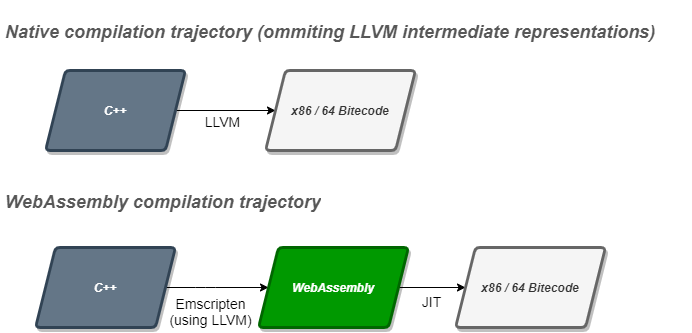
\includegraphics[width=\textwidth]{../schemas/wasm-performance/wasm-perf.png}
    \caption{Comparison of compilation trajectories. Source: Author, based on the finding of \cite{jangda_not_2019}}
    \label{fig:wasm-trajectory}
  \end{minipage}
\end{figure}

\subsubsection*{Adoption \& Implementation}

On 5 December 2019, the \ac{w3c} officially pronounced WebAssembly as the fourth programming language of the web \cite{w3c_world_2019}. Philippe Le Hégaret, the \ac{w3c} Project Lead, writes “The arrival of WebAssembly expands the range of applications that can be achieved by simply using Open Web Platform technologies. In a world where machine learning and Artificial Intelligence become more and more common, it is important to enable high performance applications on the Web, without compromising the safety of the users,”. Since then, most major browsers have added official WebAssembly support.

As of writing this proposal, WebAssembly has of yet not seen widespread adoption in web developer communities. Opinions deviate, but in general, WebAssembly is considered a niche technology, often being named as 'experimental' and 'bleeding edge'. 

This would explain why, to the best of the author's knowledge, not many projects and papers explicitly link WebAssembly and GIS. Papers on \ac{wasm} do state \textit{"3d data transformations and visualization"} as some of the examples of a high performance web applications \cite{haas_bringing_2017, jangda_not_2019}. What's more, certain GIS applications, like Google Earth, have started to use WebAssembly, as seen in \reffig{fig:google-earth} \cite{google_google_2020}. How it is used is unknown due to the engine being closed-source, but it is speculated that \ac{wasm} is used to access code written for the original C++-based desktop application.

\begin{figure}[!tbp]
  \centering
  \begin{minipage}[b]{0.80\textwidth}
    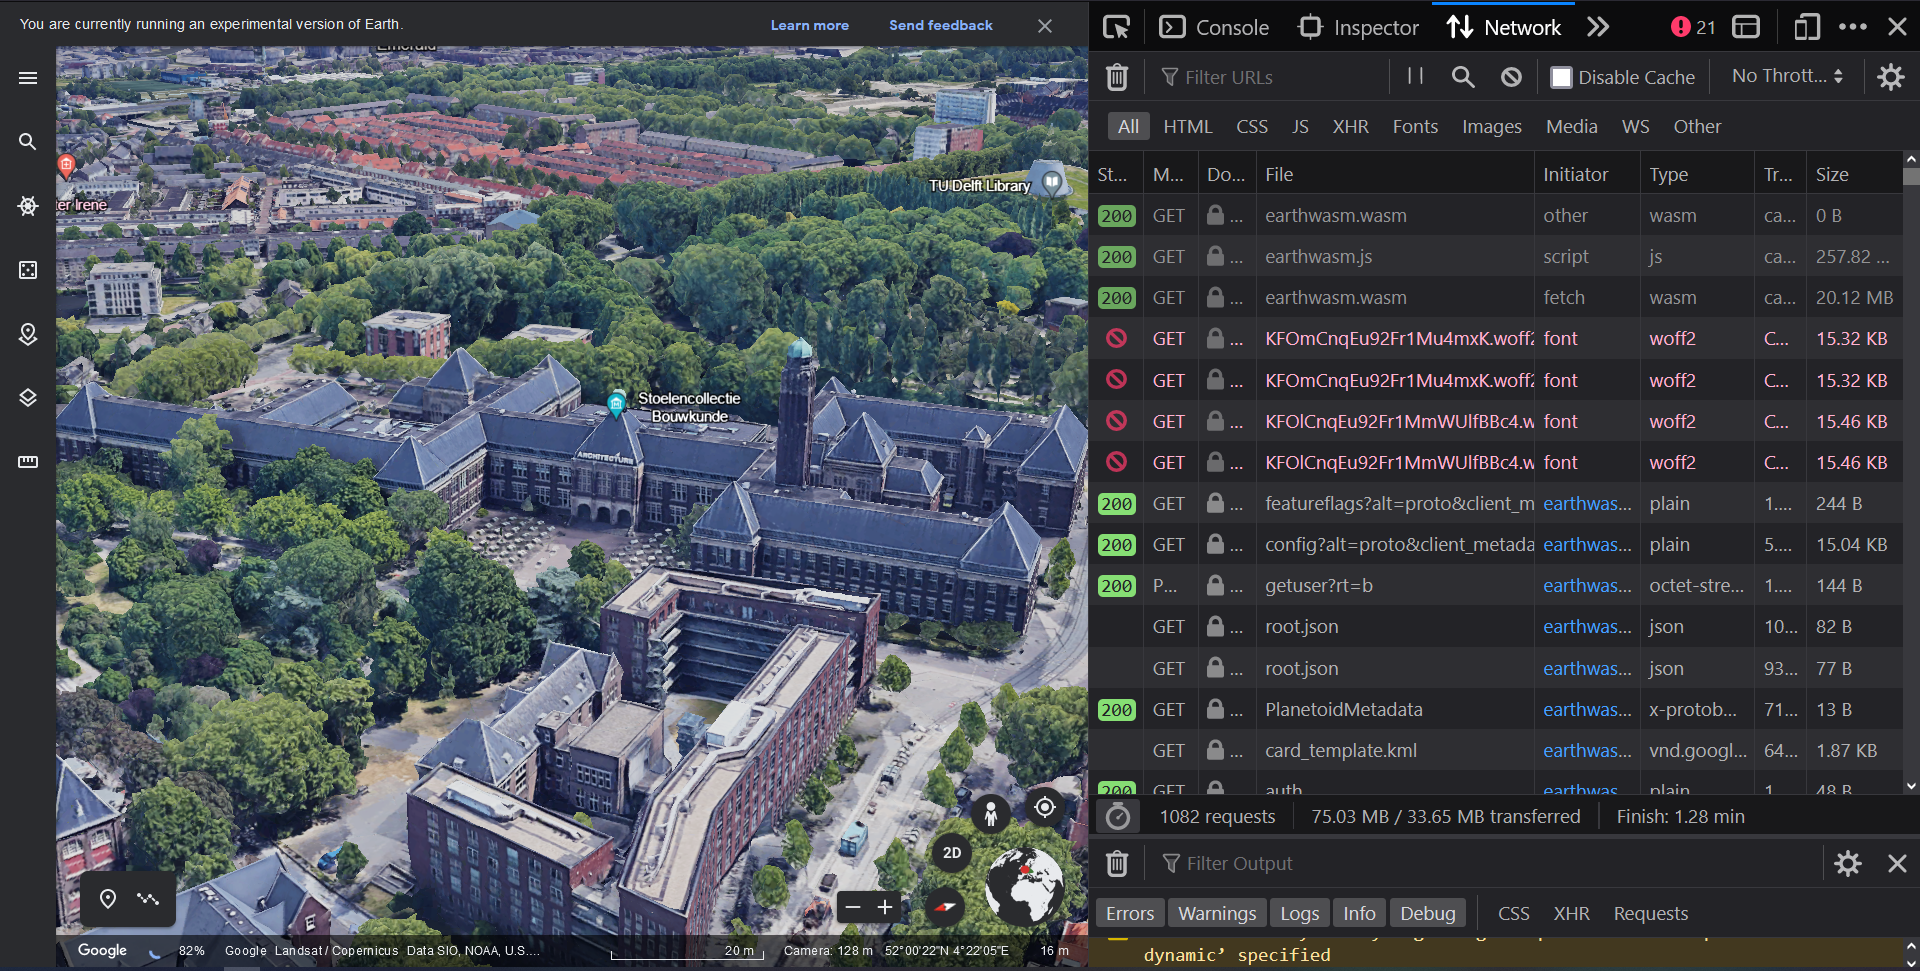
\includegraphics[width=\textwidth]{../images/google-earth-uses-webassembly.PNG}
    \caption{Google Earth utilizing WebAssembly. Source: \cite{google_google_2020}}
    \label{fig:google-earth}
  \end{minipage}
\end{figure}

Some studies have taken place evaluating \ac{wasm}'s performance for geospatial operations specifically. Melch performed extensive benchmarks on polygon simplification algorithms written in both javascript and WebAssembly \cite{melch_performance_2019}. It concludes by showing WebAssembly was not always faster, but considerably more consistent. Melch had this to say: "To call the WebAssembly code the coordinates will first have to be stored in a linear memory object. With short run times this overhead can exceed the performance gain through WebAssembly. The pure algorithm run time was always shorter with WebAssembly.". These findings match \cite{jangda_not_2019}, showing that sometimes the javascript JIT compilers of especially the chromium implementation outperform WebAssembly, mainly because of these types of linear memory overhead.

Lastly, the sparse matrix research of Sandhu et al. will be mentioned. \cite{sandhu_sparse_2018}. It shows again that WebAssembly's performance gain is most notable when performing scientific computations. it states: "For JavaScript, we observed that the best performing browser demonstrated a slowdown of only 2.2x to 5.8x versus C. Somewhat surprisingly, for WebAssembly, we observed similar or better performance as compared to C, for the best performing browser.". It also shows how certain preconceptions must be disregarded during research. For example, it turned out that for WebAssembly and JavaScript, double-precision arithmetic was more performant than single-precision.

A recent study concerned with watershed delineation \cite{sit_optimized_2019} also concluded client-side WebAssembly to be more performant than server-side C, which, as a side effect, enabled their application to be published on the web. 

%%%%%%%%%%%%%%%%%%%%%%%%%%%%%%%%%%%%%%%%%%%%%%%%%%%%%%%%%%%%%%%%%%%%%%%%%%%%%%%

\subsection{On client-side geoprocessing}

The aims of the proposed thesis also require us to be aware of previous developments in browser-based geoprocessing. 

If we forgo WebAssembly specifically, Client-side, JavaScript based geoprocessing has seen some level of academic interest throughout the last decade. The papers \cite{hamilton_client-side_2014, panidi_hybrid_2015, kulawiak_analysis_2019} all speak of an emergent trend of thick-client websites. Proponents of this trend argue that for certain applications, end users can benefit from dynamic, interactive websites which can immediately respond to a users input, rather than waiting on server round-trips necessary on static web-pages. This trend is made possible because of hardware improvements of client devices, as well as software improvements, such as HTML5. The aforementioned papers each try to apply this trend to the field of geo-informatics.

\cite{hamilton_client-side_2014} Hamilton et. al. created a such a 'thick-client', capable of replacing certain elements of server-side geoprocessing. However, the results are unfavorable towards JavaScript. It states: "The results indicated that the server was faster than the client in all testing scenarios, and only when processing generalized small scale data, was the client performance in an acceptable time range. These results demonstrated that the current implementation of web browsers are limited in their ability to execute JavaScript geoprocessing and not yet prepared to process data sizes larger than about 7,000 to 10,000 vertices before either prompting an unresponsive script warning in the browser or potentially losing the interest of the user.". While these findings are insightful, they are not directly applicable to the efforts of this study proposal. Three reasons for this:

\begin{itemize}
  \item The paper stems from 2014. Since then, javascript has seen a significant increase in performance thanks to advancements in JavaScript JIT compilers \cite{kulawiak_analysis_2019}. 
  \item The paper does not use WebAssembly, since it wasn't invented yet. The authors could have utilized 'ASM.js' \cite{mozilla_asmjs_2013} which did exist at the time, but the authors chose not to.  
  \item The paper uses an 'of the shelf', javascript library which was never designed to handle large datasets.
\end{itemize}

The same statements can be made about the the similar efforts of Panidi et. al. \cite{panidi_hybrid_2015}. However, Panidi et. al. never proposed client-side geoprocessing as a replacement of server-side geoprocessing, and spends no time on comparing the performance of the two. Instead, the authors propose a Hybrid approach, combining the advantages of server-side and client-side geoprocessing. They also present the interesting observation that client-side versus server-side geoprocessing shouldn't necessarily be a compassion of performance. "User convenience" as they put it, might dictate the usage of client-side geoprocessing in certain situations, despite speed considerations \cite{panidi_hybrid_2015}. 

%

This concern the general web community would label as \ac{ux}, is shared by a third paper \cite{kulawiak_analysis_2019}. Their article examine the current state of web-technologies from the point of view of developing cost-effective Web-GIS applications. 



% The last decade has seen a rapid evolution of processing, analysis and visualization of freely available geographic data using Open Source Web-GIS. In the beginning, Web-based Geographic Information Systems employed a thick-client approach which required installation of platform-specific browser plugins. Later on, research focus shifted to platform-independent thin client solutions in which data processing and analysis was performed by the server machine. More recently, however, the rapid development of computer hardware as well as software technologies such has HTML5 has enabled the creation of platform-independent thick clients which offer advanced GIS functionalities such as geoprocessing. 

% This article aims to analyse the current state of Open Source technologies and publicly available geographic data sources in the context of creating cost-effective Web-GIS applications for integration and processing of spatial data. 

% For this purpose the article discusses the availability and potential of Web-GIS architectures, software libraries and data sources. The analysis of freely available data sources includes a discussion of the quality and accuracy of crowd-sourced as well as public sector data, while the investigation of software libraries and architectures involves a comparison of server-side and client-side data processing performance under a set of real-world scenarios. The article concludes with a discussion of the choice of cost-effective Web-GIS architectures, software libraries and data sources in the context of the institution and environment of system deployment.

- Timely nature. Performance must be disregarded, as javascript has seen incredible improvements in the last five years \cite{haas_bringing_2017, sandhu_sparse_2018}

- These papers can, however, tell us a lot about the desires and case for client-side geoprocessing.



%%%%%%%%%%%%%%%%%%%%%%%%%%%%%%%%%%%%%%%%%%%%%%%%%%%%%%%%%%%%%%%%%%%%%%%%%%%%%%%

% VAT: A Scientific Toolbox for Interactive Geodata Exploration

\subsection{Interface \& The Geoweb}

% Line of reasoning: 
%
% - Geo-informatics papers on geoprocessing UX are not very impressive (in my humble opinion)
% - Geo-informatics papers on SDI UX and geodata as a whole are impressive 
%                                || 
%                                \/                            
% - Extend the conclusions of these papers to geoprocessing 
% - Make this the starting point of all UX reasoning within the study
%                                || 
%                                \/
% - The FAIR principles & Ilse's idea of 'community inclusivity' dictate the creation of a user friendly VPL


Finally, this proposal wishes to examine the state of the art of studies regarding geoprocessing interfaces. Unfortunately, most studies concerned specifically with geodata processing interfaces have a one to one relationship between application and interface. most papers do not state general GIS user interface principles. At the same time, general UI studies are too broad, and while insightful, the scope is too big. 

(Therefore, we stay close to home, and instead base interface considerations on topic SDI research \& geoweb)

(interesting links can be made between)

A noteworthy paper on this topic is Van den Brink's phd titled "Geospatial Data on the Web". Van den Brink states that geodata remains useful exclusively to experts in the field, despite all efforts to improve accessibility. 
She then presents the case for opening up geodata to a wider audience and more communities: "An important set of present-day users can be called “data users”: web developers, data journalists etc. who use different kinds of data, including geospatial data, directly to create applications or visualizations that supply information to end users (citizens). In order to achieve the wide re-use of geospatial data across communities, data should be easily accessible by these data users.". She also mentions the concept of FAIR geodata. Coined by \cite{mark_d_wilkinson_fair_2016}, The FAIR principles are a collection of four well-established assessment criteria used for judging the usability of (scientific) data: Findable, Accessible, Interoperable, and Reusable. 

This proposed thesis acknowledges these concepts and concerns. 
It therefore extends the idea of "community inclusively" and the concept of FAIR geodata to geoprocessing itself. 
This thesis aims to make its proposed software as Findable, Accessible, Interoperable, and Reusable as possible. 

It is for these reasons that the topic of user interface will be part of this thesis. 

UI : as Findable, Accessible, Interoperable, and Reusable as possible. 

open, cross community, base on both web, w3c standards and OGC.

for these reasons, VPL chosen, so even non-programmers



\subsubsection*{VPL}

- Ravi?

Lots of research has been done on the topic of VPL's, and their advantages and disadvantages. 
(I explicitly want to name the cognitive dimentions paper, it is very good and appropriate, and contains many suggestions for future VPL's)


% WebAssembly has the potential to improve all four of those criteria for software. If an application is published on the web without login requirements, makes it so there is no difference between Findability and Accessibility. As soon as it can be found, it can be accessed. 

% Additionally, \ac{wasm} is created explicitly to make software more \textit{Interoperable} and \textit{Reusable}.
% A ac{wasm} compiled library will work the same, wherever it is run. It is a manifestation of the  
% \textit{Write once, use anywhere} paradigm, not completely unrelated to the \textit{Collect once, use multiple times} paradigm, as both aim to minimize redundancy.



%%%%%%%%%%%%%%%%%%%%%%%%%%%%%%%%%%%%%%%%%%%%%%%%%%%%%%%%%%%%%%%%%%%%%%%%%%%%%%%


To the best of the author's knowledge, no papers exist coupling VPL to geoprocessing.

Still, this is being done, evident by...


Examination of multiple VPLS:






\subsection{Conclusion}

A conclusion can be made from every topic presented. 

On the topic of WebAssembly, the most important conclusion to to take away from prior research is \ac{wasm} must not be regarded as a 'drop-in replacement', as \cite{melch_performance_2019} puts it. Just like any language, WebAssembly has strengths and weaknesses. While \ac{wasm} is designed to be as unassumptious and unopinionated about its source language as possible, the implementations of host environments do favor certain programming patterns and data structures over others, and this will have to be taken into account during the proposed thesis.

Based on the topic of client-side geospatial processing, we can state that web technologies contain a very important temporal component. All research can become outdated, but performance analysis of web technologies are especially subject to change.  

From the category of 
- UI details important
- performance is not everything
- 'missing link'
- solving wasm issues with interface


